\chapter{実装}
\label{chap:zisso}

%ーーーーーーーーーーーーーーーーーーーーーーーーーーーー

\section{実装環境}
本研究での実装環境は下記である. 

\begin{itemize}
 \item オペレーティングシステム
    \begin{itemize}
      \item Mac OS Ventura 13.4.1
    \end{itemize}
 \item 実装言語
    \begin{itemize}
      \item Python 3.11.6
    \end{itemize}
\end{itemize}

%ーーーーーーーーーーーーーーーーーーーーーーーーーーーー

\section{スクレイピング}\label{scraping}
\subsection{Google Playストアのスクレイピング}
本研究で取得するレビュー情報は先行研究\cite{kawatsura}に合わせて下記とする. 

\begin{itemize}
 \item reviewId : レビューID
 \item userName : ユーザ名
 \item userImage : ユーザのプロフィール画像
 \item at : 投稿日時
 \item score : 星の数
 \item content : レビュー内容
 \item thumbsUpCount : このレビューが参考になったと評価した人の数
 \item reviewCreatedVersion : レビュー時のバージョン
 \item replyContent : 開発者からの返信の内容
 \item repliedAt : 開発者からの返信日時
\end{itemize}

先行研究では投稿日時が2021年10月21日〜2021年12月15日までの8週間のレビューを収集している. 収集されたGoogle Playストアの各アプリのレビュー数は表\ref{tb:rawreviewnum}の通りである. 
\begin{table}[H]
  \caption{収集したGoogle Playストアのレビュー数 (2021/10/21〜2021/12/15) ( \cite{kawatsura} p.16, 表 4.2)}
  \label{tb:rawreviewnum}
  \begin{center}
  \begin{tabular}{l|r}
    \hline
    アプリ名&収集したレビュー数(件)\\\hline\hline
    にゃんトーク&171\\\hline
    スマートニュース&1,651\\\hline
    PayPay&1,052\\\hline
    Coke ON&1,736\\\hline
    Google Fit&372\\\hline
    Simeji&468\\\hline
    Lemon8&72\\\hline
    楽天ペイ&480\\\hline
    majica&706\\\hline
    LINE MUSIC&359\\\hline
    BuzzVideo&375\\\hline
    ファミマのアプリ&290\\\hline
    CapCut&180\\\hline\hline
    合計&7,912
  \end{tabular}\end{center}
\end{table}

\noindent
この先行研究のデータに加え, 本研究では2023年10月1日〜2023年12月22日のレビューを新たに取得する. 新たに取得されたGoogle Playストアの各アプリのレビュー数を表\ref{tb:rawreviewnum2023}に示す. 
\begin{table}[H]
  \caption{収集したGoogle Playストアのレビュー数 (2023/10/1〜2023/12/22) }
  \label{tb:rawreviewnum2023}
  \begin{center}
  \begin{tabular}{l|r}
    \hline
    アプリ名&収集したレビュー数(件)\\\hline\hline
    にゃんトーク&11\\\hline
    スマートニュース&531\\\hline
    PayPay&700\\\hline
    Coke ON&840\\\hline
    Google Fit&192\\\hline
    Simeji&164\\\hline
    Lemon8&122\\\hline
    楽天ペイ&606\\\hline
    majica&128\\\hline
    LINE MUSIC&115\\\hline
    ファミマのアプリ&295\\\hline
    CapCut&263\\\hline\hline
    合計&3,967
  \end{tabular}\end{center}
\end{table}

Google PlayストアのレビューをスクレイピングするためにPythonのプログラムである\verb|get_google_play_review.py|を作成した. 
作成したプログラムの概要を次に示す. 

\begin{enumerate}
  \item アプリのパッケージ名, 言語, 取得する数, 順序を指定してレビューの一覧を取得
  \item レビュー一覧のうち指定した期間内のレビューのみを絞り込む
  \item 本論文で取得するレビュー情報のみをcsv形式で保存
\end{enumerate}
このプログラムは, レビューを取得するために, Pythonのライブラリであるgoogle-play-scraperを使用している. 
google-play-scraperでは外部依存関係なしでPython用のGoogle Playストアを簡単にクロールするためのAPIが提供されている\cite{google-play-scraper}. 

%ーーーーーーーーーーーーーーーーーーーーーーーーーーーー

\subsection{Twitterのスクレイピング}
\label{sec:x}
本研究で取得するツイート情報は先行研究\cite{kawatsura}に合わせて下記とする. 
\begin{itemize}
 \item id : ツイートID
 \item content : ツイート内容
 \item at : ツイート日時
\end{itemize}

先行研究では投稿日時が2021年10月21日〜2021年12月15日までの8週間のツイートを収集している. 収集されたTwitterの各アプリのツイート数を表\ref{tb:rawtweetnum}に示す. 

\begin{table}[H]
  \caption{収集したTwitterのツイート数 (2021/10/21〜2021/12/15) ( \cite{kawatsura} p.18, 表 4.3)}
  \label{tb:rawtweetnum}
  \begin{center}
  \begin{tabular}{l|r}
    \hline
    アプリ名&収集したツイート数(件)\\\hline\hline
    にゃんトーク&2,525\\\hline
    スマートニュース&50,590\\\hline
    PayPay&880,319\\\hline
    Coke ON&84,424\\\hline
    Google Fit&13,496\\\hline
    Simeji&205,327\\\hline
    Lemon8&4,376\\\hline
    楽天ペイ&11,111\\\hline
    majica&3,649\\\hline
    LINE MUSIC&184,873\\\hline
    BuzzVideo&41,656\\\hline
    ファミマのアプリ&8,867\\\hline
    CapCut&33,998\\\hline\hline
    合計&1,525,211
  \end{tabular}\end{center}
\end{table}

\noindent
この先行研究のデータに加え, 本研究では2023年10月1日〜2023年12月22日のツイートを新たに取得する. 新たに取得したTwitterのツイート数を表\ref{tb:rawtweetnum2023}に示す. 

\begin{table}[H]
  \caption{収集したTwitterのツイート数 (2023/10/1〜12/22) }
  \label{tb:rawtweetnum2023}
  \begin{center}
  \begin{tabular}{l|r}
    \hline
    アプリ名&収集したツイート数(件)\\\hline\hline
    にゃんトーク&27\\\hline
    スマートニュース&2,575\\\hline
    PayPay&3,297\\\hline
    Coke ON&2,595\\\hline
    Google Fit&2,760\\\hline
    Simeji&2,579\\\hline
    Lemon8&2,593\\\hline
    楽天ペイ&2,591\\\hline
    majica&2.596\\\hline
    LINE MUSIC&2,580\\\hline
    ファミマのアプリ&2,575\\\hline
    CapCut&2,592\\\hline\hline
    合計&29,360
  \end{tabular}\end{center}
\end{table}

Twitterのツイート取得に関してはTwitter APIを使用してスクレイピングを行う. Twitter APIのプランに関してはFree, Basic, Pro, Enterpriseの4つのプランが用意されており, それぞれ料金や使用できる機能などが異なる. 大規模なサービスやビジネス向けのEnterpriseプラン以外の3つのプランの違いの一部を表\ref{tb:xplan}に示す. 

\begin{table}[H]
  \caption{プランとできること}
  \label{tb:xplan}
  \begin{center}
  \begin{tabular}{l|c|c|c}
    \hline
    &Free&Basic&Pro \\\hline\hline
    料金&無料&月額100ドル&月額5,000ドル \\\hline
    月間ツイート数の上限&1,500件&3,000件&300,000件 \\\hline
    月間ツイート取得数&0件&10,000件&1,000,000件 \\\hline
  \end{tabular}\end{center}
\end{table}
表\ref{tb:xplan}よりツイートを取得するためにはBasicプラン以上に加入する必要がある. Basicプランに加入した場合でも合計で30,000件しか取得できないため, データセットの不足を補うため本研究では先行研究のデータセットを追加で使用することとした. Twitterの利用規約によると, Twitterが提供するインターフェイスを介して行うスクレイピング以外は禁止としている. そのため, seleniumなどを使用したスクレイピングは行わなかった.  

Twitter APIを使用してツイートを取得するためにPythonのプログラムである\verb|get_tweet.py|を作成した. このプログラムではTwitter APIにアクセスするためのライブラリであるTweepy\cite{tweepy}を使用した. 
実装したプログラムの概要を次に示す.
\begin{enumerate}
  \item APIキーなどの5つの認証情報をセット
  \item Clientクラスのsearch\_resent\_tweetsメソッドを使用してツイートを取得
  \item 検索ワードを含むツイート情報のうち本論文で取得する情報のみをcsv形式で保存
\end{enumerate}
先行研究と同じ情報を取得するために, 本研究ではsearch\_resent\_tweetsメソッドの引数として次に示すものを与えた. 
\begin{itemize}
 \item max\_result : 検索結果の最大数. 10〜100の数値で, デフォルトは10
 \item query: 検索ワード
 \item tweet\_field: リスト形式でツイートフィールドを選択. 今回はツイート日時を取得するために["created\_at"]とした
 \item end\_time: 期間の終わりを指定できる (UTCタイムスタンプ) 
\end{itemize}
search\_resent\_tweetsメソッドは最大で過去7日間まで遡ってツイートを取得できる. search\_all\_tweetsメソッドでは全てのツイートを取得できるが, Academic Researchアクセスの利用資格があるものしか使用できない. このアクセスを利用するにはAcademic Research申請を提出する必要があり, ``修士課程の学生, 博士号取得候補者, 博士研究員, 大学教員, 学術機関または大学の研究員である''ことが申し込みをする1つの条件となっている\cite{academic-research}. 
私は申し込みの条件を満たしていないため,本研究ではsearch\_resent\_tweetsメソッドを使用した. 

%ーーーーーーーーーーーーーーーーーーーーーーーーーーーー

\section{前処理}\label{preprocessing}
レビューに含まれるキーフレーズの自動抽出の精度を上げるために, Google PlayストアとTwitterから取得したデータに対して前処理を行うプログラム (\verb|preprocessing_google.py|, \verb|preprocessing_twitter.py|) を作成した. このプログラムでは次に示す処理を行う. 処理は一般的な自然言語処理の手法を参考としている. 
\begin{itemize}
  \item 英語を全て小文字に揃える
  \item 次に示すの文字列を削除
    \begin{itemize}
      \item 「」【】() () 『』
      \item @@から始まるメンション
      \item \#から始まるタグ
      \item URL
      \item 半角空白,全角空白
      \item 絵文字
      \item 日本語を含まないレビュー
    \end{itemize}
  \item レビューやツイートには, 異なる欠陥の報告やアプリに対する要望に関する文が2文以上からなるものがある. そのため, 「。」「.」「!」「!」「?」「!」「\verb|\n|」「\verb|\r\n|」でそれぞれの文に分割する. 
\end{itemize}
図\ref{fig:preprocessing}がレビューを前処理した例である. 2つの文で構成されているため「。」で区切り分割している. また絵文字は削除されている. 

\begin{figure}[H]
 \centering
 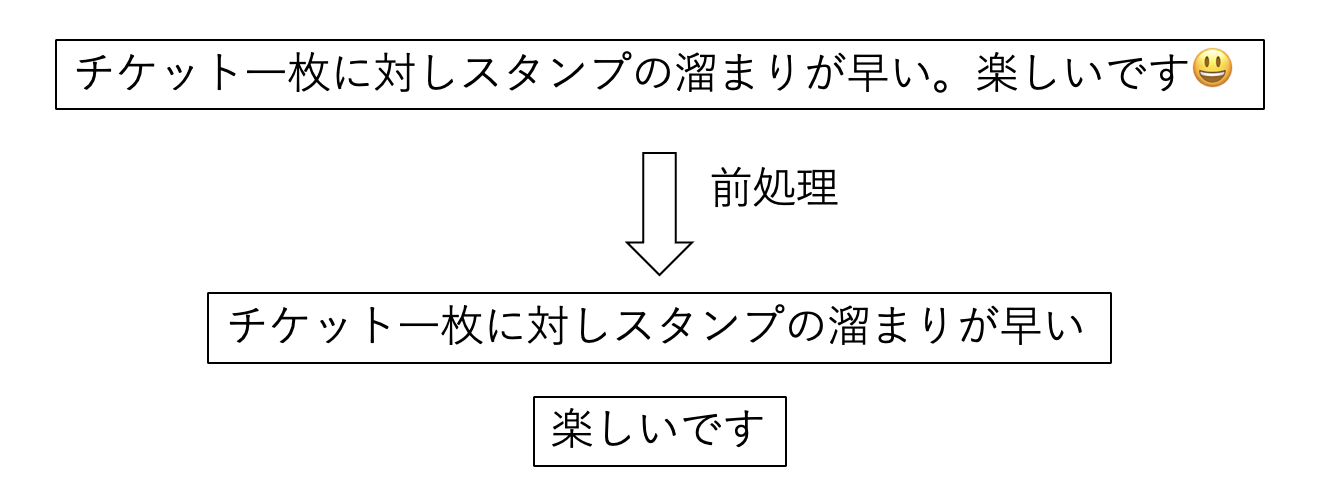
\includegraphics[scale=0.5]
      {contents/images/preprocessing.png}
 \caption{前処理の例\label{fig:preprocessing}}
\end{figure}

最後に, 前処理した結果をcsvファイルに保存する. 
表\ref{tb:googlecsv}, 表\ref{tb:twittercsv}に前処理した結果を格納するcsvファイルの一部を示す. 

\begin{table}[H]
  \caption{レビューの前処理結果 (BuzzVideo) }
  \label{tb:googlecsv}
  \begin{center}
  \begin{tabularx}{\linewidth}{|l|l|X|}
    \hline
    at&reviewId&content\\\hline\hline
    2021-12-15 19:25:30&gp:AOqpTOHj6w ...&バズビデオを見て、感動をありがとう\\\hline
    2021-12-15 12:28:09&gp:AOqpTOHleV ...&内容が残酷で異常な人が多い\\\hline
    2021-12-15 11:09:50&gp:AOqpTOHG7O ...&分かりづらい\\\hline
    2021-12-14 15:16:33&gp:AOqpTOGWvT ...&ばず29さいって人が投稿してる動画すべて虚偽動画なのでアカウント削除と動画削除して欲しい\\\hline
    2021-12-14 15:16:33&gp:AOqpTOGWvT ...&あるだけで大迷惑です\\\hline
    2021-12-14 15:16:33&gp:AOqpTOGWvT ...&二度と登録し直せないよう個体識別番号で縛ってください\\\hline
    2021-12-14 15:16:33&gp:AOqpTOGWvT ...&お願いします\\\hline
  \end{tabularx}\end{center}
\end{table}

\begin{table}[H]
  \caption{ツイートの前処理結果 (BuzzVideo) }
  \label{tb:twittercsv}
  \begin{center}
  \begin{tabularx}{\linewidth}{|l|l|X|}
    \hline
    at&id&content\\\hline\hline
    2021-12-15T23:55:11.000Z&1471267626655825922&芸能人に似てる気がするけど名前が思い出せない\\\hline
    2021-12-15T23:53:43.000Z&1471267256659509249&驚愕男性が豆乳を飲むべき3つの理由\\\hline
    2021-12-15T23:53:43.000Z&1471267256659509249&男だからこそ注目したい豆乳のメリットとは\\\hline
    2021-12-15T23:53:17.000Z&1471267149746679813&感情を乗せた歌声と歌詞に聞き惚れちゃう♪壊れかけのradio\\\hline
    2021-12-15T23:53:10.000Z&1471267120264904705&kkと眞子の酷い嘘\\\hline
    2021-12-15T23:53:10.000Z&1471267120264904705&恐ろしい真実が明らかに\\\hline
  \end{tabularx}\end{center}
\end{table}
保存する項目は, 投稿日時 (at) , レビューのid (reviewId) またはツイートid (id) , そして, 前処理した文章である. 
1つのレビュー, ツイートをいくつかの文に分割した場合には同じreviewId, idが割り振られる. 

%ーーーーーーーーーーーーーーーーーーーーーーーーーーーー

\section{キーフレーズの自動抽出}\label{extraction}
\subsection{データセット}\label{dataset}
モデルのファインチューニングに使用されるデータセットとして, Google PlayストアとTwitterのツイートからそれぞれ5,000件ずつ合計で10,000件のデータをランダムに抽出し手作業でキーフレーズを抽出した. データセットの作成は情報工学科の学部4年生2人がそれぞれ手作業で行い, お互いの抽出したキーフレーズが異なっていたものは議論することにより統一した. 
データセットには前処理したデータが格納されたcsvファイルを利用して, 抽出したキーフレーズを含めた新たなcsvファイルを作成する. 作成されたcsvファイルにはid, アプリ名, 投稿日時, 本文, 抽出したキーフレーズの5つのデータが入っている. idは前処理したデータを識別するために与えられ, Google Playストアのレビューはg\_ (index) , Twitterのツイートのidはt\_ (index) とする.  indexには各データに応じた番号が振られている. 
10,000件のデータセットのうち, 6,000件を訓練データ, 2,000件を検証用データ, 2,000件をテストデータとする. 質問応答形式のファインチューニングを行うために, csv形式であるデータセットをソースコード\ref{json}に示すようにjson形式に変換する. 

\begin{lstlisting}[caption=データセット.json,label=json]
  {
    "version": "v2.0", 
    "data": [
      {
        "title": "モバイルアプリのレビュー", 
        "paragraphs": [
          {
            "context": "本アカウントのフォローやリツイートお願いします",
            "qas": [
              {
                "id": "t_2223388",
                "question": "この文はTwitterのツイートです。
                             paypayアプリの欠陥やpaypayアプリに対する
                             要望が書かれているのはどこですか?",
                "is_impossible": true,
                "plausible_answers": [{"text": "", "answer_start": -1}],
                "answers": [{"text": "", "answer_start": -1}]
              }
            ]
          },
          {
            "context": "11/25前後からアプリを開いても強制終了、
                      会員バーコードもクーポンも何も出せない状態、
                      これでは買い物ができないと、こちらのレビュー
                      を見に来て沢山の方が同じ状態であることが
                      わかった",
            "qas": [
              {
                "id": "g_6041", 
                "question": "この文章はGooglePlayストアのレビューです。
                            majicaアプリの欠陥やmajicaアプリに対する
                            要望が書かれているのはどこですか?",
                "answers": [{"text": "アプリを開いても強制終了、
                                      会員バーコードもクーポン
                                      も何も出せない", 
                             "answer_start": -1}], 
                "is_impossible": false
              }
            ]
          }, ...
        ]
      }
    ]
  } 
\end{lstlisting}
\noindent
このjsonファイルは次に示す要素によって構成される. 

\begin{itemize}
  \item version: バージョンを表す. 本研究で用意したデータセットはSQuAD 2.0と同じバージョンであるため, v2.0とする (詳細は後述)
  \item title: contextのタイトル
  \item paragraphs: 1つのcontextとそれに関連する質問, 答えがリスト形式で保持されている
  \item qas: 質問と回答がリスト形式となっている
  \item context: 元の文章 (抽出する前の文章) 
  \item id: 設定したid
  \item question: 質問文
  \item is\_impossible: 答えられない質問ならtrue, それ以外はfalse
  \item plausible\_answers: 質問が答えられない時のみ存在し, 問題文から答えになりうる部分を抽出
  \item answers: contextから抜き出したキーフレーズとその位置情報がリスト形式で保持されている. キーフレーズを複数用意することもできる
  \item text: contextから抜き出したキーフレーズのテキスト
  \item answer\_start: contextから抜き出したキーフレーズの位置情報
\end{itemize}

ここでSQuADとは質問応答タスクで一般的に使用されているスタンフォード質問回答データセットである. 
SQuADにはv1.1とv2.0という2つのバージョンがある. v1.1は全ての質問が回答可能で, v2.0では答えられない質問が含まれる. 本研究ではキーフレーズが含まれないレビューも存在し, SQuAD 2.0と同じ形式であるため, v2.0としている. 

\subsection{モデルのファインチューニング}
用意したデータセットを用いて事前学習済みモデルをファインチューニングする. 本研究では事前学習済みモデルとしてHugging FaceのTransformersを通して利用できる東北大学のモデル\cite{tohoku}を使用する. このモデルは日本語のWikipediaのデータを用いて学習されている\cite{tohoku}. 
この東北大学が公開している日本語BERTのうち, whole word maskingを適用して学習させているモデル\cite{masking}を用いる. whole word maskingとは事前学習時に単語ごとでマスクするかどうかを決め, マスクする単語に対応するサブワードを全てマスクする方式である. モデルのパラメータは次に示す通りである. 
\begin{itemize}
  \item 学習率: 3e-5
  \item エポック数: 10
  \item バッチサイズ: 12
\end{itemize}
実装にはTransformersに含まれるスクリプトであるrun\_squad.pyを用いる. 

\subsection{キーフレーズの自動抽出}
作成した自動抽出モデルを使用して, 前処理したGoogle PlayストアとTwitterのデータからキーフレーズを自動抽出する. 自動抽出を行うexecute\_answer関数をソースコード\ref{answer}に示す. 
\begin{lstlisting}[caption=execute\_answer関数,label=answer]
# モデルとトークナイザーの準備
model = AutoModelForQuestionAnswering.from_pretrained('output/')  
tokenizer = BertJapaneseTokenizer.from_pretrained('cl-tohoku/bert-base-japanese-whole-word-masking') 

def execute_answer(context, question):
    # 自動抽出の実行
    inputs = tokenizer.encode_plus(question, context, add_special_tokens=True, return_tensors="pt")
    input_ids = inputs["input_ids"].tolist()[0]
    output = model(**inputs)
    answer_start = torch.argmax(output.start_logits)  
    answer_end = torch.argmax(output.end_logits) + 1 
    answer = tokenizer.convert_tokens_to_string(tokenizer.convert_ids_to_tokens(input_ids[answer_start:answer_end]))
    answer = answer.replace(" ", "")

    del inputs, output
    torch.cuda.empty_cache()

    return answer
\end{lstlisting}
このソースコードの実行フローを次に示す.  

\begin{enumerate}
  \item ファインチューニングを行ったモデルとトークン化を行うためのBERT用トークナイザーを準備 (2, 3行目)
  \item 質問文と抽出対象のデータをトークナイザーでトークン化し, モデルへの入力データ (inputs) を作成 (7行目)
  \item トークン化された文章のidをリスト (input\_ids) に変換 (8行目)
  \item 作成した入力データを使ってモデルに入力し, 出力 (output) を取得 (9行目)
  \item 抽出したキーフレーズのトークンの開始位置と終了位置を取得 (10, 11行目)
  \item 開始位置から終了位置までのトークンを文字列に変換してキーフレーズ (answer) を取得 (12行目)
\end{enumerate}
結果はid, アプリ名, 投稿日時, 文章, 抽出したキーフレーズをcsv形式で保存する. 保存されたcsvファイルの一部を表\ref{tb:googleqa}に示す. 

\begin{table}[H]
  \caption{レビューの自動抽出結果}
  \label{tb:googleqa}
  \small
  \begin{center}
  \begin{tabularx}{\linewidth}{l|l|X|X|X}
    \hline
    id&アプリ名&投稿日時&元のレビュー&抽出したキーフレーズ\\\hline\hline
    g\_955&coke\_on&2021-11-27 11:17:03&商品が出ない事が何回か発生しました&商品が出ない\\\hline
    g\_959&coke\_on&2021-11-11 15:32:50&そもそも自販機側が黄色点滅していなくて買えないことが多過ぎです&自販機側が黄色点滅していなくて買えない\\\hline
    g\_961&coke\_on&2021-11-14 23:13:26&今まではcoke\_on対応を優先してかっていたが、これからはコカコーラ製品全般をできるだけ買わないようにする&今まではcoke\_on対応を優先してかっていたが、これからはコカコーラ製品全般をできるだけ買わないようにする\\\hline
    g\_964&coke\_on&2021-10-24 12:30:07&自販機との接続を早くしてほしい&自販機との接続を早くしてほしい\\\hline
  \end{tabularx}\end{center}
\end{table}

表\ref{tb:googleqa}からわかるように, ``自販機との接続を早くしてほしい''という元のレビューから``自販機との接続を早くしてほしい''というキーフレーズを抽出するなど, 元のレビューがそのままキーフレーズとして抽出されることがある. 

%ーーーーーーーーーーーーーーーーーーーーーーーーーーーー

\section{クラスタリング}\label{clustering}
\subsection{ベクトルの生成}
抽出した文章をその文章が示す意味に応じてクラスタリングする. クラスタリングをするために日本語Sentence-BERTクラスを定義する. 日本語Sentence-BERTクラス (SentenceBertJapanese) の各関数の概要を示す. 
\begin{itemize}
  \item \_\_init\_\_関数 : モデルとトークナイザーの初期化を行う
  \item \_mean\_pooling関数 : モデルの出力とAttention Maskを用いて, 文の埋め込みを生成するための平均プーリングを行う
  \item encode関数 : 文のリストから各文章の埋め込みを求める
\end{itemize}

このように, 日本語BERT用にファインチューニングしたBERTを用いて各トークンの埋め込みを求め, 平均を取ることにより文全体の埋め込みを求めている. 

% sentence-bertクラス
% \begin{lstlisting}[caption=clustering.py,label=sentence-bert]
%   class SentenceBertJapanese:
%     def __init__ (self, model_name_or_path, device=None) :
%         self.tokenizer = BertJapaneseTokenizer.from_pretrained (model_name_or_path) 
%         self.model = BertModel.from_pretrained (model_name_or_path) 
%         self.model.eval () 

%         if device is None:
%             device = "cuda" if torch.cuda.is_available ()  else "cpu"
%         self.device = torch.device (device) 
%         self.model.to (device) 

%     def _mean_pooling (self, model_output, attention_mask) :
%         token_embeddings = model_output[0] #First element of model_output contains all token embeddings
%         input_mask_expanded = attention_mask.unsqueeze (-1) .expand (token_embeddings.size () ) .float () 
%         return torch.sum (token_embeddings * input_mask_expanded, 1)  / torch.clamp (input_mask_expanded.sum (1) , min=1e-9) 

%     @torch.no_grad () 
%     def encode (self, sentences, batch_size=8) :
%         all_embeddings = []
%         iterator = range (0, len (sentences) , batch_size) 
%         for batch_idx in iterator:
%             batch = sentences[batch_idx:batch_idx + batch_size]

%             encoded_input = self.tokenizer.batch_encode_plus (batch, padding="longest", 
%                                            truncation=True, return_tensors="pt") .to (self.device) 
%             model_output = self.model (**encoded_input) 
%             sentence_embeddings = self._mean_pooling (model_output, encoded_input["attention_mask"]) .to ('cpu') 

%             all_embeddings.extend (sentence_embeddings) 

%         # return torch.stack (all_embeddings) .numpy () 
%         return torch.stack (all_embeddings) 
% \end{lstlisting}
%
% \begin{lstlisting}[caption=clustering.py,label=model]
%   model = SentenceBertJapanese ("sonoisa/sentence-bert-base-ja-mean-tokens") 
% \end{lstlisting}

SentenceBertJapaneseクラスの引数に日本語モデル名を与えることによりインスタンスが生成され, モデルの読み込みが完了する. このインスタンスを使用して抽出されたキーフレーズをベクトルに変換する. 

\subsection{グラフクラスタリング}
次に, それぞれの抽出したキーフレーズをノード, ノードのベクトル間のコサイン類似度をエッジとする無向グラフを作成する. 

作成されたグラフからChinese Whispersによりグラフクラスタリングが実行される. クラスタリングを実行するcw関数をソースコード\ref{cw}に示す. 

\begin{lstlisting}[caption=cw関数,label=cw]
  def cw (input_csv_file, category, app_name) :
    sentences = create_review_list (input_csv_file, app_name) 
    sentence_vectors = model.encode (sentences) 
    domain_docs = {f'{app_name}': sentences}
    threshold = 0.8
    clusters = []
    
    doc_embeddings = compute_embeddings (domain_docs) 
    G = create_graph (doc_embeddings, threshold, sentence_vectors) 
    # Perform clustering of G, parameters weighting and seed can be omitted
    chinese_whispers (G, weighting='top', iterations=20) 
    for node in G.nodes () :
        text = str (G.nodes[node]['text']) 
        label = int (G.nodes[node]['label']) 
        clusters.append ([text, label]) 
\end{lstlisting}

このソースコードの実行フローを次に示す. 

\begin{enumerate}
  \item モデルを使用して文のベクトル表現 (sentence\_vectors) を生成 (3行目) 
  \item Chinese Whispersで使用される閾値 (threshold) , 抽出したキーフレーズとクラスタ番号を格納する2次元配列 (clusters) を用意 (5, 6行目)
  \item create\_graph関数を使用し, グラフを作成. 引数には文の埋め込み, 閾値, 文のベクトル表現を与える (9行目)
  \item chinese\_whispers関数の引数に作成されたグラフ, エッジの重み付けを決定する方法 (詳細は後述) , Chinese Whispersアルゴリズムの反復回数を与えて実行
  \item chinese\_whispers関数の実行によりグラフの各ノードに抽出されたキーフレーズ (text) とクラスタ番号 (label) が格納されているためfor文で各情報をclusterに格納していく (12行目〜15行目)
\end{enumerate}

本研究ではエッジの重み付けを決定する方法はデフォルトのtop (エッジの重みをそのまま使用する方法) にし, エッジの最大トークンが重みとして使用される. また, 反復回数は20とした. 

クラスタリングした結果, それぞれの文章にクラスタを識別する番号 (以下 : クラスタ番号) が振られる. クラスタ番号が同じものが同じクラスタとなり, クラスタ番号が近いものは意味的相関が近いことを表す. ノード間のコサイン類似度スコアの閾値を決めることで, どの程度類似した文章を同じクラスタとして定義するのかが決定される. 
結果はcsvファイルに保存される. 表\ref{tb:clustering}に示されるように抽出したキーフレーズにそれぞれクラスタ番号が振られる. 

\begin{table}[H]
  \caption{抽出したキーフレーズとクラスタ番号 (google\_fit) }
  \label{tb:clustering}
  \begin{center}
  \begin{tabularx}{\linewidth}{X|r}
    \hline
    抽出したキーフレーズ&cluster\\\hline\hline
    再起動しても直らない&275\\\hline
    接続/連携を適宜確認しておく必要がある&276\\\hline
    歩いた歩数より足りない&279\\\hline
    使えない&280\\\hline
    使えない&280\\\hline
    歩けない&280\\\hline
    使えない&280\\\hline
    動かなかった&280\\\hline
    反応しない&280\\\hline
    使い方も分からない&280\\\hline
    使えない&280\\\hline
    使えない&280\\\hline
    動かなくなった&280\\\hline
    長期放置されてるんでしょうか&281\\\hline
    下がるって何故でしょうか&282\\\hline
    カウントされなくなる&283\\\hline
    何もカウントしなくなった&283\\\hline
    カウント出来ていない&283\\\hline
    カウントされず&283\\\hline
    記録ができませんと&283\\\hline
  \end{tabularx}\end{center}
\end{table}

\subsection{クラスタ名の決定}
KeyBERTのキーワード抽出によりクラスタ名を決定する手法について説明する. 作成したkeybert関数をソースコード\ref{keybert}に示す. 

\begin{lstlisting}[caption=keybert関数, label=keybert]
  # spaCyの初期化(日本語モデルを使用)
  nlp = spacy.load ('ja_ginza') 

  # 日本語BERTモデルの読み込み
  keybertmodel = SentenceTransformer ('cl-tohoku/bert-base-japanese') 
  keybert_model = KeyBERT (model=keybertmodel) 

  def keybert (text) :
    # spaCyを使用して名詞, 固有名詞, 動詞, 形容詞, 数詞を抽出
    doc = nlp (text) 
    tokens = [token.text for token in doc if token.pos_ == ''NOUN'' or token.pos_ == ''PROPN'' or token.pos_ == ``ADJ'' or token.pos_ == ``NUM'' or token.pos_ == ``VERB'']
    # tokensをKeyBERTに渡してキーワード抽出
    tokens_text = `` ''.join (tokens) 
    keywords = keybert_model.extract_keywords (tokens_text, top_n = 3, keyphrase_ngram_range= (1, 1) , stop_words=None) 
    title = ``''
    for title_word in keywords:
        title = title + ``【'' + title_word[0] + ``】 ''
    return title
\end{lstlisting}

このソースコードの実行フローを次に示す. 

\begin{enumerate}
  \item クラスタの各キーフレーズを結合した1つの大きな文書 (text) をトークン化する (10行目)
  \item トークンのうち名詞, 固有名詞, 動詞, 形容詞, 数詞のみを含む配列を作成 (11行目)
  \item この配列を`` '' (空白) で結合し, 新たな文書を生成 (13行目)
  \item KeyBERTモデルのインスタンスからキーワードを抽出するメソッド (extract\_keywords) を呼び出し, キーワードを配列で取得. メソッドの引数には抽出対象となる文書, 抽出するキーワードの数, キーワードの長さを与える. (14行目)
  \item キーワードからクラスタ名を生成し, 返す (15行目〜18行目)
\end{enumerate}

クラスタ名が決定したら, クラスタ番号とクラスタ名の組み合わせを格納したcsvファイルを作成する. 

%ーーーーーーーーーーーーーーーーーーーーーーーーーーーー

\section{可視化}\label{display}
\subsection{使用した言語・フレームワーク}
可視化ツールの実装に使用した言語, フレームワークは次に示す通りである. 
\begin{itemize}
    \item フロントエンド: HTML/CSS, JavaScript
    \item バックエンド: Python
    \item フレームワーク: Flask
\end{itemize}

\subsection{概要}
レビューをマイニングした結果を開発者が分析しやすくするためにwebブラウザ上で表示する. 表示する際はクラスタごとにまとめて表示することで類似したレビューはまとめて閲覧できるようになっている. 
そして, レビューの特徴を表す2種類のグラフを用いることで, 開発者がレビューの内容や投稿日時にどのような傾向があるかを把握しやすくなっている. また, 期間やキーワードで検索できるような機能を入れているためレビューを条件に応じて絞り込むことができる. 

\subsection{画面構成}
画面は大きく分けて一覧画面とアプリごとの詳細画面の2つからなる. 

一覧画面では次に示す項目や機能を表示, 付与する. 

\begin{itemize}
  \item 期間, キーワードで絞り込める検索機能
  \item 全てのアプリに対する日ごとのレビュー数を表す折れ線グラフ (Google Playストアのレビューとツイートそれぞれについて)
\end{itemize}

アプリごとの詳細画面では, 次に示す項目や機能を表示, 付与する.

\begin{itemize}
  \item 期間, キーワードで絞り込める検索機能
  \item アコーディオンメニューを使用して抽出したキーフレーズの一覧をクラスタごとに表示
  \item 抽出したキーフレーズをクリックすると投稿日時や元のレビューをモーダルウィンドウで表示
  \item 日ごとのレビュー数を表す折れ線グラフの表示
  \item クラスタに含まれるレビュー数の上位10個を表す棒グラフの表示
\end{itemize}

アプリの修正や機能の追加などを行った際に, ユーザがアプリの変更に対してどのような内容のレビューを挙げているか, レビュー数に変化があるかどうかを確認することはアプリの開発にとって非常に重要であると考えられる. 
したがって, 本研究で実装した可視化ツールには日ごとのレビュー数を表す折れ線グラフや, クラスタに含まれるレビュー数の上位10個を表す棒グラフを表示している. 
この2つのグラフによって, 開発者は``レビューの投稿が多い日''や``どのような内容のレビューを多くの人が投稿しているか''を把握することができる. 
また, 特定の機能や期間に関するレビューだけを確認したい際には検索機能を使用してレビューを絞り込むことができる. 
これらの機能によって膨大な数があるレビューを開発者が確認する負担を軽減し, レビューを分析する効率を向上させることができる. 

google fitのレビュー一覧の表示が図\ref{fig:review_items}である. 

\begin{figure}[H]
  \centering
  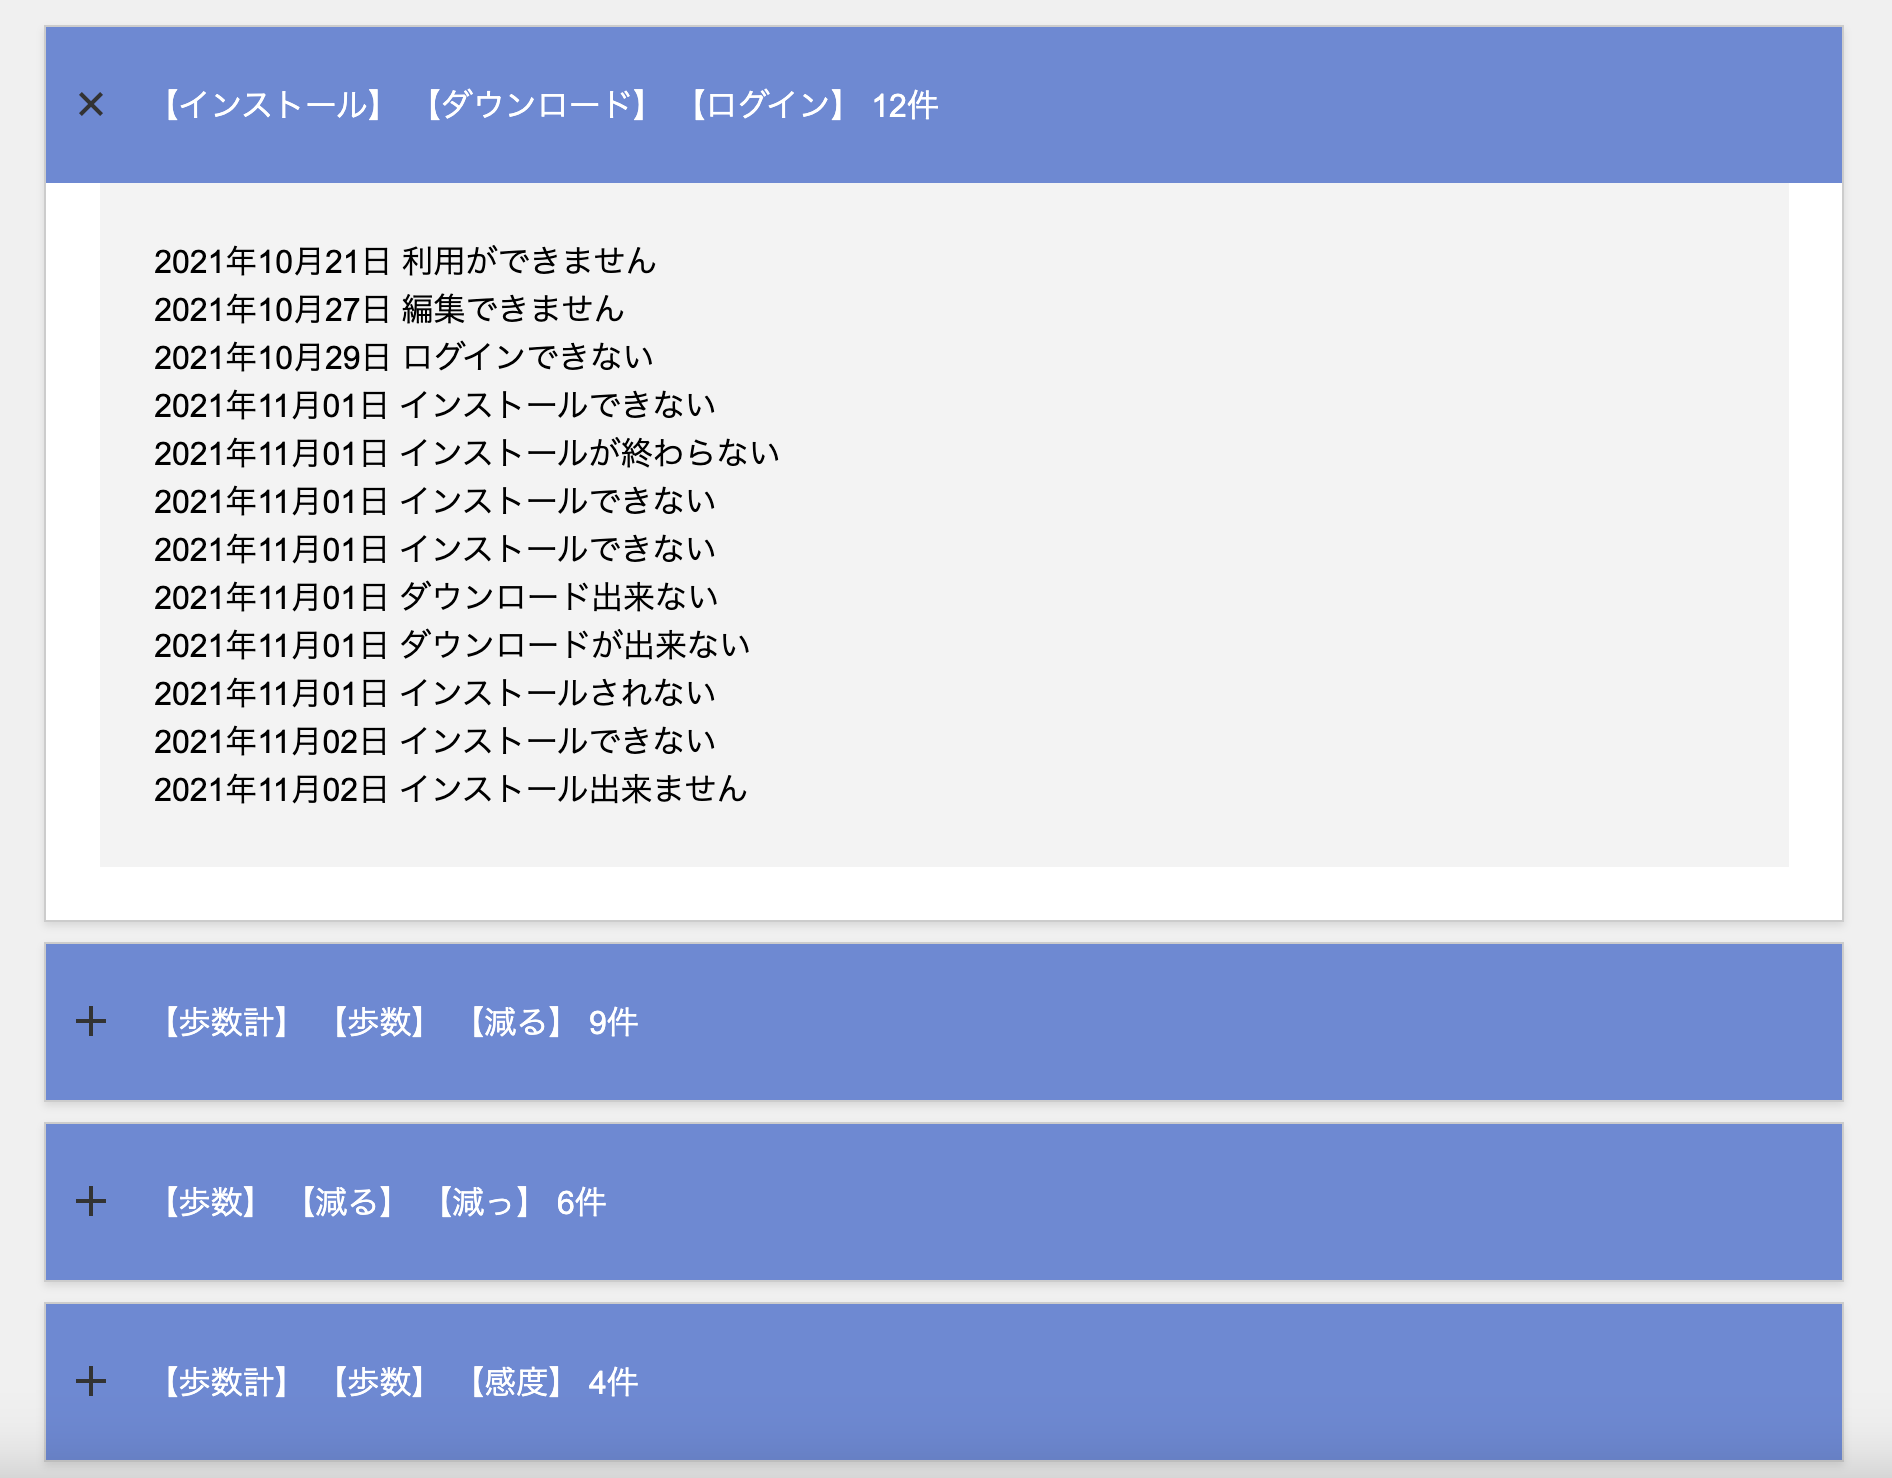
\includegraphics[scale=0.3]
    {contents/images/review_items.png}
  \caption{google fitのレビュー一覧\label{fig:review_items}}
\end{figure}

\noindent
この一覧はクラスタに含まれるレビュー数が多いものから順に表示されており, ページネーションによって1つのページでレビュー100件ごと表示している. 
初期状態では, クラスタ名のみ表示されており, クラスタ名をクリックするとアコーディオンメニューが開き, そのクラスタに属するレビューの一覧が表示される. アコーディオンメニュー内では投稿された日付と抽出されたキーフレーズのみ表示されるが, 抽出されたキーフレーズをクリックすると投稿日時, レビューの全文, 抽出したキーフレーズがモーダルで表示される (図\ref{fig:modal}). 
クラスタごとに表示し, 類似したレビューをまとめることで開発者がレビューを確認する効率を上げることができる. 

\begin{figure}[H]
  \centering
  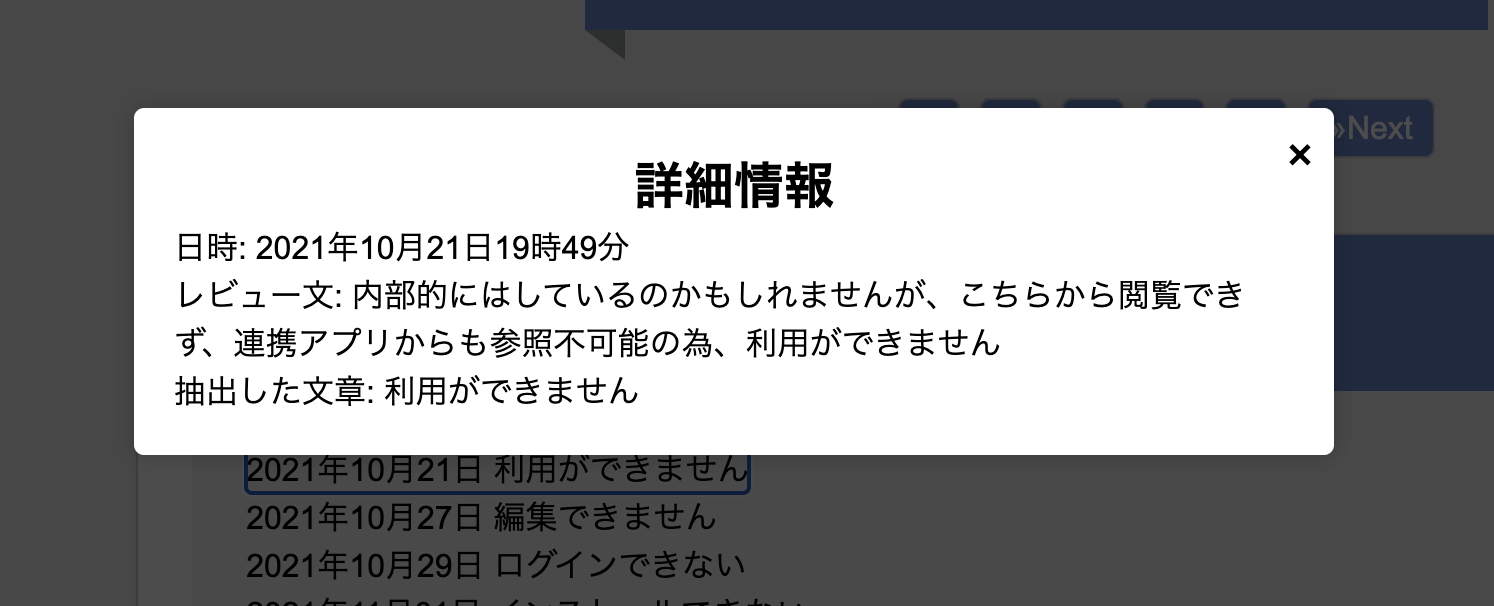
\includegraphics[scale=0.5]
    {contents/images/modal.png}
  \caption{レビューのモーダル表示\label{fig:modal}}
\end{figure}

\subsection{検索のロジック}
ページの検索欄で期間とキーワードを入力すると指定した期間, キーワードと一致するレビューのみをページに表示させることができる. 
検索結果をページに反映させるためのソースコード\ref{search}を示す. 

\begin{lstlisting}[caption=view.py, label=search]
  # ファイル読み込み, 日付でソートしたリスト作成
  with open ('該当アプリのcsvファイルの相対パス', 'r', encoding='utf-8-sig')  as csv_file:
      csv_reader = csv.reader (csv_file) 
      rows = list (csv_reader) 
      rows = sorted (rows, reverse=False, key=lambda x:x[2]) 

  # 検索結果のリスト作成
  search_result = []
  for row in rows:
      if start_date <= row[2][:10] <= end_date:
          if keyword != "":
              if keyword in row[3]:
                  search_result.append (row) 
          else:
              search_result.append (row) 
  rows = search_result
\end{lstlisting}

このソースコードの実行フローを次に示す. 

\begin{enumerate}
  \item 抽出, クラスタリングが行われた結果を格納したcsvファイルを開き, リスト形式に変換する (1行目〜5行目)
  \item 各レビューの投稿期間が検索で指定した期間の範囲内にあるかどうかを確認する (10行目)
  \item 検索で指定したキーワードがないなら, そのまま検索結果を格納するリスト (search\_list) に格納する(11, 14, 15行目)
  \item 検索で指定したキーワードがある場合, レビューがそのキーワードを含む場合は検索結果を格納するリスト (search\_list) に格納する (11行目〜13行目)
\end{enumerate}

\subsection{グラフの作成}
グラフの作成にはplotly.jsを用いる. plotly.jsとはグラフ生成ライブラリであり, 3Dグラフや統計グラフなど40を超えるグラフタイプが同梱されている\cite{plotly}.
plotly.jsで作成されたグラフにはオプションとしてズーム機能やグラフのダウンロード機能が付随している. 
日付ごとのレビュー数に関するグラフを表示するソースコード\ref{graph}を示す. 

\begin{lstlisting}[caption=detail.html, label=graph]
  <div class="graph-title">日付ごとのレビュー数の推移</div>
  <div id="scatter"></div>

  <script>
      // 横軸: 日付
      var labels = JSON.parse ('{{ graphs | map (attribute=0)  | list | tojson | safe }}') ;
      // ラベル用日付
      var displayLabels = [];
      for  (var i = 0; i < labels.length; i += 5)  {
          displayLabels.push (labels[i]) ;
      }
      var values = JSON.parse ('{{ graphs | map (attribute=1)  | list | tojson | safe }}') ;

      var data = [{
          x: labels,
          y: values,
          type: 'scatter',
      }];

      var layout = {
          title: '日付ごとのレビュー数の推移',
          height: 600,
          width: 1200,
          xaxis: {
              tickvals: displayLabels,  // 配列の5つおきの目盛り位置を指定
          }
      };

      Plotly.newPlot ('scatter', data, layout) ;
  </script>
\end{lstlisting}

このソースコードの実行フローを次に示す. 

\begin{enumerate}
  \item DOMのターゲットを設定する (2行目)
  \item graphsからレビューが投稿された日付を取得し, 配列 (labels) を生成する (6行目)
  \item グラフの横軸に表示する日付のみを格納したリスト (displayLabels) を生成する (8行目〜11行目)
  \item graphsから日付ごとのレビュー数を取得し, 配列 (values) を生成する (12行目)
  \item 横軸に日付, 縦軸にその日付に投稿されたレビュー数を表示する折れ線グラフを生成するための変数 (data) を宣言する (14行目〜18行目)
  \item タイトルやグラフのサイズ, 横軸に表示する内容を指定するための変数 (layout) を宣言する (20行目〜27行目)
  \item JavaScriptのPlotlyライブラリにあるnewPlotメソッドでグラフを生成する. 引数には, DOMのターゲットのid, 宣言済みのdata, layoutを渡す (20行目〜27行目)
\end{enumerate}
ここでgraphsはレビューが投稿された日付とその日のレビュー数が格納された二次元リストである. この二次元リストはバックエンド側で作成される. 
横軸にレビューが投稿された日付, 縦軸にレビュー数を取るグラフである. 
dataのtypeでグラフタイプを指定でき, layoutでタイトルや表の大きさを指定できる. 

ソースコード\ref{graph}によって作成されたグラフが図\ref{fig:majica_graph}である. このグラフは, majicaのレビューにおける日付とレビュー数の関係を表した折れ線グラフである. 
横軸がレビューが投稿された日付, 縦軸がレビュー数をそれぞれ表している. 

\begin{figure}[H]
  \centering
  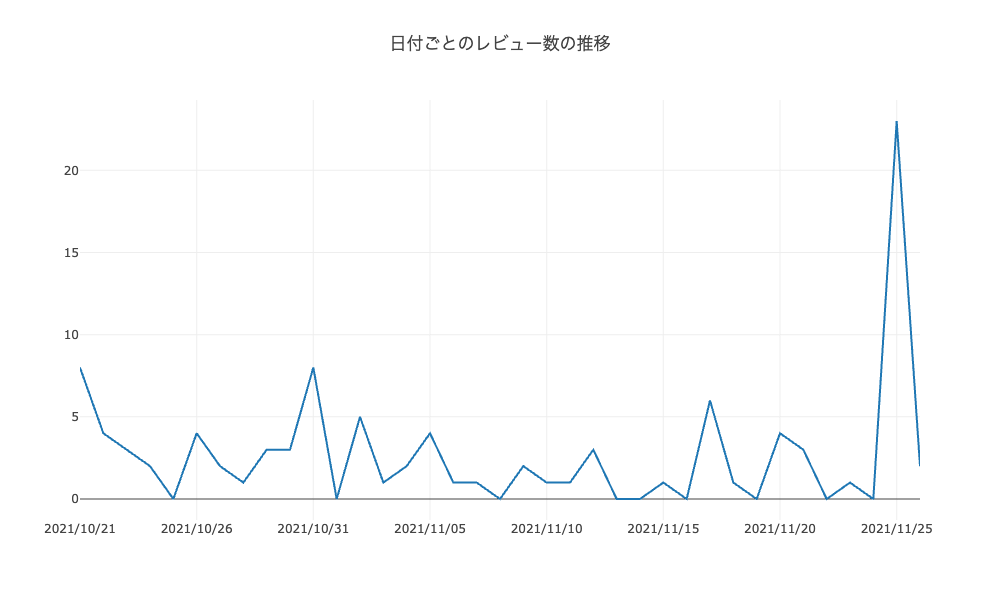
\includegraphics[scale=0.4]
    {contents/images/majica_graph.png}
  \caption{majicaのレビューにおける日付とレビュー数の関係\label{fig:majica_graph}}
\end{figure}

このグラフを閲覧することでいつ多くのレビューが挙げられているかどうか確認することができる. また, 検索結果に対応してグラフの日付やレビュー数が変更されるようになっている. 
図\ref{fig:majica_graph}より, majicaのレビューは11月25日に多くのレビューが挙げられていることがわかる. そして11月25日のレビューの内容を詳細画面で確認すると, ``更新したらアプリが開けない'', ``更新してから開けなくなりました''といったアプリの更新による不具合が多く報告されていることがわかった. 
このレビューをもとに開発者は更新の内容や起動時のコードなどを確認し, 早急に修正を行うと考えられる. 

クラスタに含まれるレビュー数の上位10個を表す棒グラフが図\ref{fig:top10}である. 横軸がクラスタ名, 縦軸がレビュー数をそれぞれ表している. 
このグラフはGoogle Fitにおけるクラスタのうちレビュー数が多いものを10個表示している. 

\begin{figure}[H]
  \centering
  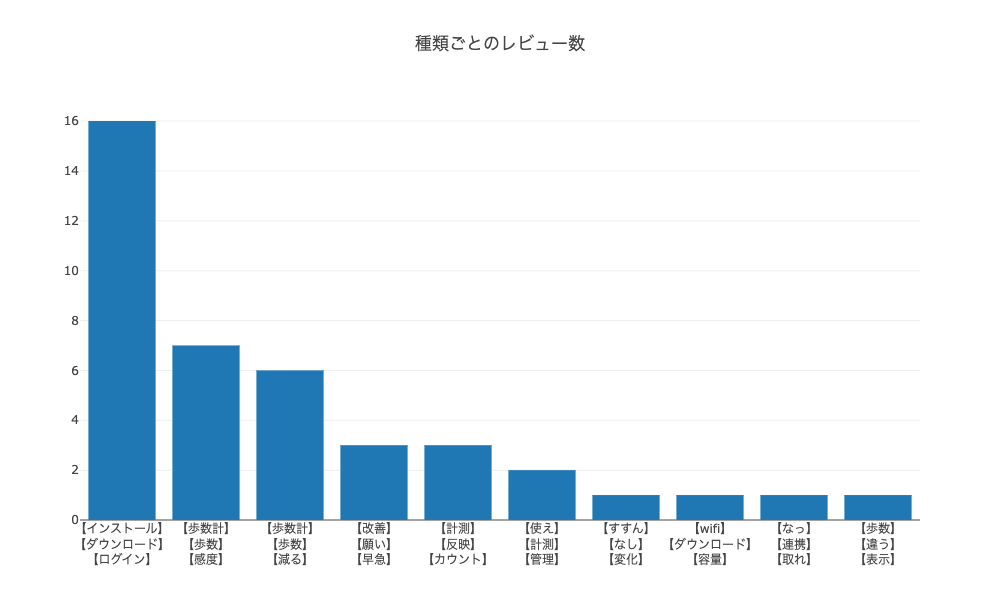
\includegraphics[scale=0.4]
    {contents/images/top10.png}
  \caption{Google Fitのレビューにおけるクラスタごとのレビュー数\label{fig:top10}}
\end{figure}

このグラフを確認すると, インストールやログインに関する不具合や歩数が減少してしまう不具合を報告するレビューが多いことがわかる. このように1つ1つのレビューを確認しなくてもどのような内容のレビューが多く投稿されているのかが可視化されている. 
そして, このグラフも検索結果に対応して, 各クラスタに含まれるレビュー数が変更されるようになっている. 
